\documentclass[11pt,letterpaper,twoside]{article}
\usepackage[english]{babel}
\usepackage{amssymb,amsmath}
\usepackage{fancyhdr}
\usepackage{graphicx}
\usepackage{wrapfig}

 \oddsidemargin  0in \evensidemargin 0in
 \topmargin   -0.25in \headheight 0.25in \headsep 0.25in
 \textwidth   6.5in \textheight 8.75in \marginparsep 0pt \marginparwidth 0pt
 \parskip 1ex  \parindent 0ex \footskip 20pt

\newfont{\bssten}{cmssbx10}
\newfont{\bssnine}{cmssbx10 scaled 900}

%%%%%%%%%%%%%%%%%%%%%%%
\newcommand{\whatizit}{Lecture 13: The Geometric Distribution}
%%%%%%%%%%%%%%%%%%%%%%%


\pagestyle{fancy}  
\fancyhead{\bssnine STOR 155,  \whatizit}
\fancyhead[RE]{} \fancyhead[LO]{}
\fancyhead[LE]{\bssnine \thepage} \fancyhead[RO]{\bssnine \thepage}
\lfoot{} \cfoot{} \rfoot{}   


\newcommand{\var}{\mathrm{Var}}



\begin{document}



\thispagestyle{empty} \vspace*{-0.75in}

{\bssten STOR 155: Introduction to Data Models and Inference \hfill June 5, 2024 \\
Prof. Will Lassiter  \hfill Page 1 of \pageref{totalpag}}
\vspace{10pt}
\begin{center} {{\Large \bf \whatizit}} \end{center}

Running example: the Milgram experiment \vspace{6pt}

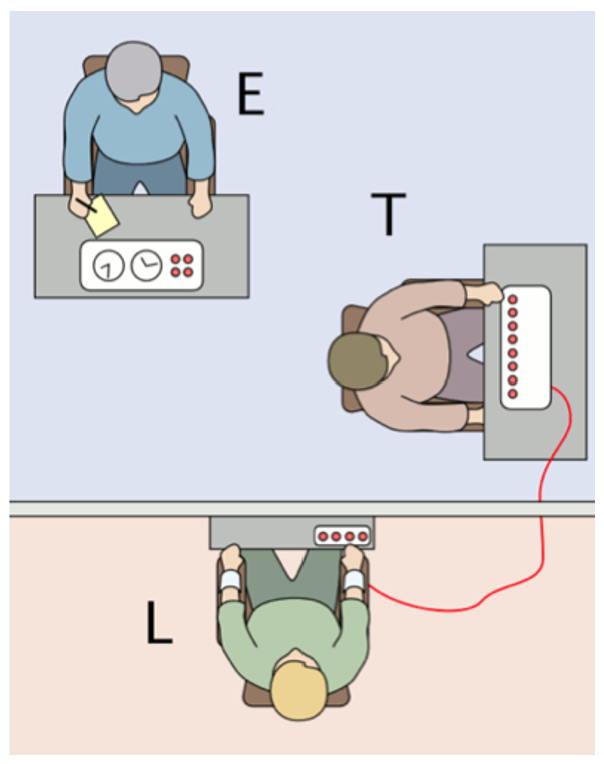
\includegraphics[scale=0.8]{images/milgram.png} \vspace{20pt}

{\bf The Bernoulli Distribution}

\newpage

Example: Roll a fair six-sided die and consider the roll a ``success" if a 2 or a 3 comes up.

\vspace{120pt}

{\bf The Geometric Distribution} \vspace{6pt}

Dr.\ Mario wants to repeat Milgram's experiment, but he only wants to sample people until he finds someone who will not inflict a severe shock. What is the probability that he stops after ...

\begin{itemize}

\item ... the first person? \vspace{40pt}

\item ... the third person? \vspace{40pt}

\item ... the tenth person? \vspace{40pt}

\end{itemize}

The geometric distribution describes ... \vspace{120pt}

Possible values and probabilities:

\newpage

Example: Probability that it will take 6 rolls of a fair six-sided die to produce the first 6? \vspace{60pt}

Expected Value and Variance for a Geometric Random Variable \vspace{240pt}

Example: back to Milgram experiment \vspace{120pt}

Example: back to rolling a 6 with a fair die

\newpage

More interesting example: Suppose there is an 85\% chance it will not rain on any given day, independent of all other days. 

\begin{itemize}

\item Given that it rains today, what is the probability that it will rain again tomorrow? \vspace{60pt}

\item Calculate the mean and standard deviation for the number of days until we see rain again. \vspace{120pt}

\item Which future day (relative to today) is most likely to be the next day we see rain?

\end{itemize}

\label{totalpag}
\end{document}
